\usetikzlibrary{arrows.meta}
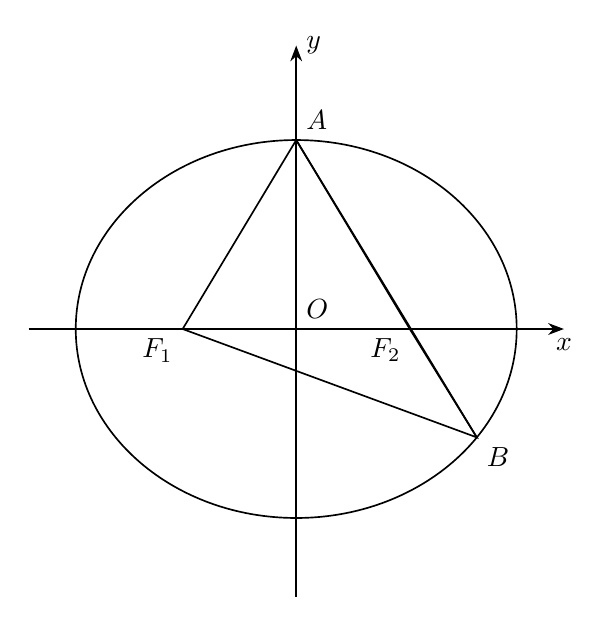
\begin{tikzpicture}[line width=.6pt,font=\normalsize,>=Stealth]
\coordinate (O) at (0,0);
\coordinate (A) at (0,2.4);
\coordinate (Fone) at (-1.44222051,0);
\coordinate (Ftwo) at (1.44222051,0);
\coordinate (B) at (2.293625724,-1.376583447);
\draw[->] (-3.4,0) -- (3.4,0) node[below] {$x$};
\draw[->] (0,-3.4) -- (0,3.6) node[right] {$y$};
\draw (O) ellipse (2.8 and 2.4);
\draw (A) -- (Fone) -- (B) -- (A);
\draw (A) -- (Ftwo) -- (B);
\node[above right] at (A) {$A$};
\node[below left] at (Fone) {$F_{1}$};
\node[below left,inner sep=3pt] at (Ftwo) {$F_{2}$};
\node[below right] at (B) {$B$};
\node[above right] at (O) {$O$};
\end{tikzpicture}
